\subsection{Set Operations} \label{sec:setOperations}
\logToConsole{SET OPERATIONS}

The reachability algorithms implemented in CORA rely on set-based computation. One major design principle is that the same standard set operations are implemented for all set representations so that algorithms can be executed with different set representations. In this section, we introduce the most important set operations, which are demonstrated by examples involving concrete set representations. Set representations are later detailed in \cref{sec:setRepresentations}; however, in order to follow the subsequent examples, it suffices to consider the sets as arbitrary continuous sets.

If a set representation is not closed under an operation, an over-approximation is returned (see \cref{tab:basicOperations}).

\subsubsection{Basic Set Operations}

We first consider basic operations on sets.

\subsubsubsection{mtimes}
\label{sec:mtimes}

The method \operator{mtimes}, which overloads the * operator, implements the linear map of a set. Given a set $\mathcal{S} \subset \R^n$, the linear map is defined as 
\begin{equation*}
	\operator{mtimes}(M,\mathcal{S}) = M \otimes \mathcal{S} = \{ M s ~|~ s \in \mathcal{S} \},~ M \in \mathbb{R}^{w \times n}.
\end{equation*}
It is also possible to consider a set of matrices $\mathcal{M} \subset \R^{w \times n}$ instead of a fixed-value matrix $M \in \R^{w \times n}$ (see \cref{sec:mtimesMatSet}). Let us demonstrate the method $\operator{mtimes}$ by an example:

\begin{center}
\begin{minipage}[t]{0.35\textwidth}
	\vspace{10pt}
	\footnotesize
	\definecolor{mycolor1}{rgb}{0.00000,0.44700,0.74100}%
\definecolor{mycolor2}{rgb}{0.46600,0.67400,0.18800}%
%
\begin{tikzpicture}
\footnotesize
\pgfplotsset{
plotstyle1/.style={color=mycolor1, forget plot},
plotstyle2/.style={color=mycolor2, forget plot}
}
\def\rows{1}
\def\cols{2}
\def\horzsep{1cm}
\def\basepath{./figures/tikz/matSet-operations/}

\begin{groupplot}[%
group style={rows = \rows, columns = \cols, horizontal sep = \horzsep},
scale only axis,
width=1/\cols*\textwidth -\horzsep,
legend style={legend columns=2,legend to name=legendname, legend cell align=left,/tikz/every even column/.append style={column sep=0.5cm}}
]
\nextgroupplot[xmin=-3,xmax=3,ymin=-3,ymax=3,xlabel={$x_{(1)}$},ylabel={$x_{(2)}$},title={$\mathcal{S}$}]
\input{\basepath example_mtimes_11.tikz}
\coordinate (top) at (rel axis cs:0,1);
\nextgroupplot[xmin=-3,xmax=3,ymin=-3,ymax=3,xlabel={$x_{(1)}$},title={$A\otimes\mathcal{S}$}]
\input{\basepath example_mtimes_legends.tikz}
\input{\basepath example_mtimes_12.tikz}
\coordinate (bot) at (rel axis cs:1,0);
\end{groupplot}
\path (top|-current bounding box.south)--coordinate(legendpos)(bot|-current bounding box.south);
\node at([yshift=-6ex]legendpos) {\pgfplotslegendfromname{legendname}};

\end{tikzpicture}%
\end{minipage}
\begin{minipage}[t]{0.6\textwidth}
	\vspace{0pt}
	\centering
	\includetikz{./figures/tikz/set-operations/example_mtimes}
\end{minipage}
\end{center}


\subsubsubsection{plus}
\label{sec:plus}

The method \operator{plus}, which overloads the + operator, implements the Minkowski sum of two sets. Given two sets $\mathcal{S}_1,\mathcal{S}_2 \subset \Rn$, the Minkowski sum is defined as 
\begin{equation*}
	\operator{plus}(\mathcal{S}_1,\mathcal{S}_2) = \mathcal{S}_1 \oplus \mathcal{S}_2 = \{ s_1 + s_2 ~|~ s_1 \in \mathcal{S}_1,~ s_2 \in \mathcal{S}_2 \}.
\end{equation*}
Let us demonstrate the method $\operator{plus}$ by an example:

\begin{center}
\begin{minipage}[t]{0.35\textwidth}
	\vspace{10pt}
	\footnotesize
	\input{./MATLABcode/example_plus}
\end{minipage}
\begin{minipage}[t]{0.6\textwidth}
	\vspace{0pt}
	\centering
	\includetikz{./figures/tikz/set-operations/example_plus}
\end{minipage}
\end{center}



\subsubsubsection{cartProd}
\label{sec:cartProd}

The method \operator{cartProd} implements the Cartesian product of two sets. Given two sets $\mathcal{S}_1 \subset \Rn$ and $\mathcal{S}_2 \subset \R^w$, the Cartesian product is defined as 
\begin{equation*}
	\operator{cartProd}(\mathcal{S}_1,\mathcal{S}_2) = \mathcal{S}_1 \times \mathcal{S}_2 = \{ [s_1 ~ s_2 ]^T ~|~ s_1 \in \mathcal{S}_1,~ s_2 \in \mathcal{S}_2 \}.
\end{equation*}
Let us demonstrate the method $\operator{cartProd}$ by an example:

\begin{center}
\begin{minipage}[t]{0.35\textwidth}
	\vspace{10pt}
	\footnotesize
	% This file was created by matlab2tikz.
%
\definecolor{mycolor1}{rgb}{0.00000,0.44700,0.74100}%
%
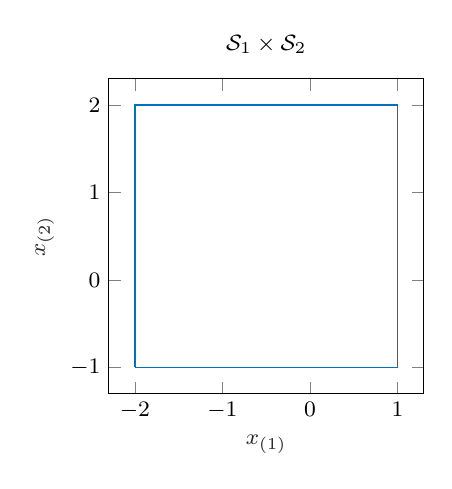
\begin{tikzpicture}
\footnotesize

\begin{axis}[%
width=4cm,
height=4cm,
at={(0in,0in)},
scale only axis,
xmin=-2.3,
xmax=1.3,
xlabel style={font=\color{white!15!black}},
xlabel={$x_{(1)}$},
ymin=-1.3,
ymax=2.3,
ylabel style={font=\color{white!15!black}},
ylabel={$x_{(2)}$},
axis background/.style={fill=white},
title style={font=\bfseries},
title={$\mathcal{S}_1\times\mathcal{S}_2$}
]
\addplot [color=mycolor1, forget plot]
  table[row sep=crcr]{%
-2	-1\\
1	-1\\
1	2\\
-2	2\\
-2	-1\\
};
\end{axis}
\end{tikzpicture}%
\end{minipage}
\begin{minipage}[t]{0.3\textwidth}
	\vspace{10pt}
	\begin{verbatim}
		Command Window:	
	
		res = 
 [-2.00000,1.00000]
 [-1.00000,2.00000]
	\end{verbatim}
\end{minipage}
\begin{minipage}[t]{0.3\textwidth}
	\vspace{0pt}
	\centering
	\includetikz{./figures/tikz/set-operations/example_cartProd}
\end{minipage}
\end{center}


\subsubsubsection{convHull}
\label{sec:convHull}

The method \operator{convHull} implements the convex hull of two sets. Given two sets $\mathcal{S}_1,\mathcal{S}_2 \subset \Rn$, the convex hull is defined as 
\begin{equation*}
	\operator{convHull}(\mathcal{S}_1,\mathcal{S}_2) = \left \{ \lambda s_1 + (1-\lambda) s_2 ~|~ s_1,s_2 \in \mathcal{S}_1 \cup \mathcal{S}_2,~\lambda \in [0,1] \right\}.
\end{equation*}
Furthermore, given a single non-convex set $\mathcal{S} \subset \Rn$, $\operator{convHull}(\mathcal{S})$ computes the convex hull of the set. Let us demonstrate the method $\operator{convHull}$ by an example:

\begin{center}
\begin{minipage}[t]{0.35\textwidth}
	\vspace{10pt}
	\footnotesize
	\input{./MATLABcode/example_convHull}
\end{minipage}
\begin{minipage}[t]{0.6\textwidth}
	\vspace{0pt}
	\centering
	\includetikz{./figures/tikz/set-operations/example_convHull}
\end{minipage}
\end{center}



\subsubsubsection{quadMap}
\label{sec:quadMap}

The method \operator{quadMap} implements the quadratic map of a set. Given a set $\mathcal{S} \subset \Rn$, the quadratic map is defined as 
\begin{equation*}
	\operator{quadMap}(\mathcal{S},Q) = \{ x ~|~ x_{(i)} = s^T Q_i s, ~s \in \mathcal{S},~ i = 1 \dots w \}, ~ Q_i \in \R^{n \times n},
\end{equation*}
where $x_{(i)}$ is the $i$-th value of the vector $x$. If \operator{quadMap} is called with two different sets $\mathcal{S}_1,\mathcal{S}_2 \subset \Rn$ as input arguments, the method computes the mixed quadratic map:
\begin{equation*}
	\operator{quadMap}(\mathcal{S}_1,\mathcal{S}_2,Q) = \{ x ~|~ x_{(i)} = s_1^T Q_i s_2, ~s_1 \in \mathcal{S}_1,~s_2 \in \mathcal{S}_2,~ i = 1 \dots w \}, ~ Q_i \in \R^{n \times n}.
\end{equation*}
Let us demonstrate the method $\operator{quadMap}$ by an example:

\begin{center}
\begin{minipage}[t]{0.35\textwidth}
	\vspace{10pt}
	\footnotesize
	\input{./MATLABcode/example_quadMap}
\end{minipage}
\begin{minipage}[t]{0.6\textwidth}
	\vspace{0pt}
	\centering
	\includetikz{./figures/tikz/set-operations/example_quadMap}
\end{minipage}
\end{center}

\vspace{1cm}

\subsubsubsection{and}
\label{sec:and}

The method \operator{and}, which overloads the \& operator, implements the intersection of two sets. Given two sets $\mathcal{S}_1,\mathcal{S}_2 \subset \Rn$, the intersection is defined as 
\begin{equation*}
	\operator{and}(\mathcal{S}_1,\mathcal{S}_2) = \mathcal{S}_1 \cap \mathcal{S}_2 = \{ s ~|~ s \in \mathcal{S}_1,~ s \in \mathcal{S}_2 \}.
\end{equation*}
Let us demonstrate the method $\operator{and}$ by an example:

\begin{center}
\begin{minipage}[t]{0.35\textwidth}
	\vspace{10pt}
	\footnotesize
	\input{./MATLABcode/example_and}
\end{minipage}
\begin{minipage}[t]{0.6\textwidth}
	\vspace{0pt}
	\centering
	\includetikz{./figures/tikz/set-operations/example_and}
\end{minipage}
\end{center}

\subsubsubsection{or}
\label{sec:or}

The method \operator{or}, which overloads the $|$ operator, implements the union of two sets. Given two sets $\mathcal{S}_1,\mathcal{S}_2 \subset \Rn$, their union is defined as 
\begin{equation*}
	\operator{or}(\mathcal{S}_1,\mathcal{S}_2) = \mathcal{S}_1 \cup \mathcal{S}_2 = \{ s ~|~ s \in \mathcal{S}_1 \vee s \in \mathcal{S}_2 \}.
\end{equation*}
Let us demonstrate the method $\operator{or}$ by an example:

\begin{center}
\begin{minipage}[t]{0.35\textwidth}
	\vspace{10pt}
	\footnotesize
	\definecolor{mycolor1}{rgb}{0.00000,0.44700,0.74100}%
\definecolor{mycolor2}{rgb}{0.85000,0.32500,0.09800}%
\definecolor{mycolor3}{rgb}{0.46600,0.67400,0.18800}%
%
\begin{tikzpicture}
\footnotesize
\pgfplotsset{
plotstyle1/.style={color=mycolor1, forget plot},
plotstyle2/.style={color=mycolor2, forget plot},
plotstyle3/.style={color=mycolor3, forget plot}
}
\def\rows{1}
\def\cols{2}
\def\horzsep{1cm}
\def\basepath{./figures/tikz/set-operations/}

\begin{groupplot}[%
group style={rows = \rows, columns = \cols, horizontal sep = \horzsep},
scale only axis,
width=1/\cols*\textwidth -\horzsep,
legend style={legend columns=2,legend to name=legendname, legend cell align=left,/tikz/every even column/.append style={column sep=0.5cm}}
]
\nextgroupplot[xmin=-3,xmax=3,ymin=-3,ymax=3,xlabel={$x_{(1)}$},ylabel={$x_{(2)}$},title={$\mathcal{S}_1$ and $\mathcal{S}_2$}]
\input{\basepath example_or_11.tikz}
\coordinate (top) at (rel axis cs:0,1);
\nextgroupplot[xmin=-3,xmax=3,ymin=-3,ymax=3,xlabel={$x_{(1)}$},title={$\mathcal{S}_1\cup\mathcal{S}_2$}]
\input{\basepath example_or_legends.tikz}
\input{\basepath example_or_12.tikz}
\coordinate (bot) at (rel axis cs:1,0);
\end{groupplot}
\path (top|-current bounding box.south)--coordinate(legendpos)(bot|-current bounding box.south);
\node at([yshift=-6ex]legendpos) {\pgfplotslegendfromname{legendname}};

\end{tikzpicture}%
\end{minipage}
\begin{minipage}[t]{0.6\textwidth}
	\vspace{0pt}
	\centering
	\includetikz{./figures/tikz/set-operations/example_or}
\end{minipage}
\end{center}


\begin{table*}
\centering
	\caption{Relations between set representations and set operations. The shortcuts e (exact computation) and o (over-approximation) are used. The symbol e* indicates that the operation is exact if no independent generators (see \cref{sec:polynomialZonotopes} and \cref{sec:conPolyZono} for details) are used.}
	\label{tab:basicOperations}
	\begin{tabular}{ p{2.5cm} C{1.4cm} C{1.4cm} C{1.4cm} C{1.4cm} C{1.4cm} C{1.4cm} C{1.4cm}}
		 \toprule
		 \textbf{Set Rep.} & \textbf{Lin. Map} & \textbf{Mink. Sum} & \textbf{Cart. Prod.} & \textbf{Conv. Hull} & \textbf{Quad. Map} & \textbf{Inter- section} & \textbf{Union} \\
		 \midrule
		 \operator{interval} & o & e & e & o &  & e & o \\
		 \operator{zonotope} & e & e & e & o & o & o & o  \\
		 \operator{polytope} & e & e & e & e &  & e & o \\
		 \operator{conZonotope} & e & e & e & e & o & e & o \\
		 \operator{zonoBundle} & e & e & e & e & o & e & o \\
		 \operator{ellipsoid} & e  & o & o & o &  & o &  \\
		 \operator{capsule} & e & o & & & & & \\
		 \operator{taylm} & e & e & e & & & & \\
		 \operator{polyZonotope} & e & e & e & e* & e* &  & \\
		 \operator{conPolyZono} & e & e & e & e* & e* & e* & e* \\
		 \bottomrule
	\end{tabular}
\end{table*}

\subsubsubsection{minkDiff}
\label{sec:minkDiff}

The method \operator{minkDiff} implements the Minkowski difference of two sets. Given two sets $\mathcal{S}_1,\mathcal{S}_2 \subset \Rn$, their Minkowski difference is defined as 
\begin{equation*}
	\operator{minkDiff}(\mathcal{S}_1,\mathcal{S}_2) = \{ s \in \R^n ~|~ s \oplus \mathcal{S}_2 \subseteq \mathcal{S}_1 \}.
\end{equation*}
Let us demonstrate the method $\operator{minkDiff}$ by an example:

\begin{center}
	\begin{minipage}[t]{0.35\textwidth}
		\vspace{10pt}
		\footnotesize
		% This file was automatically created from the m-file 
% "m2tex.m" written by USL. 
% The fontencoding in this file is UTF-8. 
%  
% You will need to include the following two packages in 
% your LaTeX-Main-File. 
%  
% \usepackage{color} 
% \usepackage{fancyvrb} 
%  
% It is advised to use the following option for Inputenc 
% \usepackage[utf8]{inputenc} 
%  
  
% definition of matlab colors: 
\definecolor{mblue}{rgb}{0,0,1} 
\definecolor{mgreen}{rgb}{0.13333,0.5451,0.13333} 
\definecolor{mred}{rgb}{0.62745,0.12549,0.94118} 
\definecolor{mgrey}{rgb}{0.5,0.5,0.5} 
\definecolor{mdarkgrey}{rgb}{0.25,0.25,0.25} 
  
\DefineShortVerb[fontfamily=courier,fontseries=m]{\$} 
\DefineShortVerb[fontfamily=courier,fontseries=b]{\#} 
  
\noindent       
 $$\color{mgreen}$% set 1 and set 2$\color{black}$$\\
 $S1 = zonotope($\color{mblue}$ ...$\color{black}$$\\
 $        [0.5 0.5 -0.3 1 0;$\color{mblue}$ ...$\color{black}$$\\
 $         0   0.2  1   0 1]);$\\
 $S2 = interval([-1;-1],[1;1]);$\\
 $$\\
 $$\color{mgreen}$% Minkowski difference$\color{black}$$\\
 $res = minkDiff(S1,S2);$\\ 
  
\UndefineShortVerb{\$} 
\UndefineShortVerb{\#}
	\end{minipage}
	\begin{minipage}[t]{0.6\textwidth}
		\vspace{0pt}
		\centering
		\includetikz{./figures/tikz/set-operations/example_minkDiff}
	\end{minipage}
\end{center}


\subsubsection{Predicates}

Predicates check if sets fulfill certain properties and return either \operator{true} or \operator{false}.

\subsubsubsection{contains}

The method \operator{contains} checks if a set is contains another set.
Given two sets $\mathcal{S}_1,\mathcal{S}_2 \subset \Rn$, the method \operator{contains} is defined as
	\begin{equation*}
		\operator{contains}(\mathcal{S}_1,\mathcal{S}_2) = 
		\begin{cases}
			\operator{true}, & \mathcal{S}_2 \subseteq \mathcal{S}_1, \\
			\operator{false} & \mathrm{otherwise}.
		\end{cases}
	\end{equation*}
In addition, the method \operator{contains} can be applied to check if a point or a point cloud (represented as a matrix whose columns are individual points) is located inside a set. For point clouds, we return the result of the containment check for each individual point in a matrix. Since containment checks can be computationally expensive, we implemented over-approximative algorithms for some set representations (see \cref{tab:in}). If the over-approximative algorithm returns \operator{true}, it is guaranteed that $\mathcal{S}_2$ is contained in $\mathcal{S}_1$. However, if the over-approximative algorithm returns \operator{false}, the set $\mathcal{S}_2$ could still be contained in $\mathcal{S}_1$. To execute the over-approximative instead of the exact algorithm, one has to add the flag 'approx':
\begin{verbatim}
	res = contains(S1,S2,'approx');
\end{verbatim}

Let us demonstrate the method $\operator{contains}$ by an example:

\begin{center}
\begin{minipage}[t]{0.40\textwidth}
	\vspace{10pt}
	\footnotesize
	\input{./MATLABcode/example_in}
\end{minipage}
\begin{minipage}[t]{0.2\textwidth}
	\vspace{10pt}

	\begin{verbatim}
	Command Window:	
		
	res1 = true
	
res2 = true
	\end{verbatim}
\end{minipage}
\begin{minipage}[t]{0.3\textwidth}
	\vspace{0pt}
	\centering
	\includetikz{./figures/tikz/set-predicates/example_contains}
\end{minipage}
\end{center}

\begin{table}[htb]
	\centering
	\footnotesize
	\caption{Containment checks $\mathcal{S}_2 \subseteq \mathcal{S}_1$ implemented by the method \operator{contains}($\mathcal{S}_1,\mathcal{S}_2$) in CORA. The column headers represent the set $\mathcal{S}_1$ and the row headers represent the set $\mathcal{S}_2$. The shortcuts e (exact check) and o (over-approximation) are used. If both, an exact and an over-approximative algorithm are implemented, we write e/o.}
	\label{tab:in}
	\begin{tabular}{ l c c c c c c c c c c c c}
		\toprule
					 & \textbf{I} & \textbf{Z} & \textbf{P} & \textbf{cZ} & \textbf{zB} & \textbf{E} & \textbf{C} & \textbf{pZ} & \textbf{cPZ} & \textbf{levelSet} \\
		\midrule
		\textbf{interval} (I)       		  & e & e/o & e & e/o & e/o & e	& e & o & o & o \\
		\textbf{zonotope} (Z)      		    & e & e/o & e & e/o & e/o & e	& e & o & o & o \\
		\textbf{polytope} (P)   	        & e & e/o & e & e/o & e/o & e	& e & o & o & o \\
		\textbf{conZonotope} (cZ)		      & e & e/o & e & e/o & e/o & e	& e & o & o & o \\
		\textbf{zonoBundle} (zB)  	      	  & e & e/o & e & e/o & e/o & e	& e & o & o & o \\
		\textbf{ellipsoid} (E)       	      & e & e   & e & e   & e   & e & o & o & o & o \\
		\textbf{capsule} (C)				  & e & e   & e & e   & e   & o	& e & o & o & o \\
		\textbf{polyZonotope} (pZ)		 	  & o & o   & o & o   & o   & o	& o & o & o & o \\
		\textbf{conPolyZono} (cPZ)			  & o & o   & o & o   & o   & o	& o & o & o & o \\
		\textbf{taylm}     	                  & o & o   & o & o   & o   & o	& o & o & o & o \\
		\bottomrule
	\end{tabular}
\end{table}



\subsubsubsection{isIntersecting}

The method \operator{isIntersecting} checks if two sets intersect. Given two sets $\mathcal{S}_1,\mathcal{S}_2 \subset \Rn$, the method \operator{isIntersecting} is defined as
	\begin{equation*}
		\operator{isIntersecting}(\mathcal{S}_1,\mathcal{S}_2) =
		\begin{cases}
			\operator{true}, & \mathcal{S}_1 \cap \mathcal{S}_2 \neq \emptyset, \\
			\operator{false} & \mathrm{otherwise}.
		\end{cases}
	\end{equation*}	
Since intersection checks can be computationally expensive, we implemented over-approximative algorithms for some set representations (see \cref{tab:isIntersecting}). If the over-approximative algorithm returns \operator{false}, it is guaranteed that the sets do not intersect. However, if the over-approximative algorithm returns \operator{true}, the sets could possibly not intersect. To execute the over-approximative instead of the exact algorithm, one has to add the flag 'approx':
\begin{verbatim}
	res = isIntersecting(S1,S2,'approx');
\end{verbatim}

Let us demonstrate the method $\operator{isIntersecting}$ by an example:

\begin{center}
\begin{minipage}[t]{0.40\textwidth}
	\vspace{10pt}
	\footnotesize
	% This file was created by matlab2tikz.
%
\definecolor{mycolor1}{rgb}{0.00000,0.44700,0.74100}%
\definecolor{mycolor2}{rgb}{0.85000,0.32500,0.09800}%
%
\begin{tikzpicture}
\footnotesize

\begin{axis}[%
width=4cm,
height=4cm,
at={(0in,0in)},
scale only axis,
xmin=-2.4,
xmax=2.4,
xlabel style={font=\color{white!15!black}},
xlabel={$x_{(1)}$},
ymin=-2.4,
ymax=2.4,
ylabel style={font=\color{white!15!black}},
ylabel={$x_{(2)}$},
axis background/.style={fill=white},
title style={font=\bfseries},
title={$\mathcal{S}_1$ and $\mathcal{S}_2$}
]
\addplot [color=mycolor1, forget plot]
  table[row sep=crcr]{%
-1	-1\\
2	-1\\
2	2\\
-1	2\\
-1	-1\\
};
\addplot [color=mycolor2, forget plot]
  table[row sep=crcr]{%
-2	-2\\
1	-2\\
1	1\\
-2	1\\
-2	-2\\
};
\end{axis}
\end{tikzpicture}%
\end{minipage}
\begin{minipage}[t]{0.2\textwidth}
	\vspace{10pt}

	\begin{verbatim}
	Command Window:
		
	res = true
	\end{verbatim}
\end{minipage}
\begin{minipage}[t]{0.3\textwidth}
	\vspace{0pt}
	\centering
	\includetikz{./figures/tikz/set-predicates/example_isIntersecting}
\end{minipage}
\end{center}

\begin{table}[htb]
	\centering
	\footnotesize
	\caption{Intersection checks implemented by the function \operator{isIntersecting}($\mathcal{S}_1,\mathcal{S}_2$) in CORA. The shortcuts e (exact check) and o (over-approximation) are used. If both, an exact and an over-approximative algorithm are implemented, we write e/o.}
	\label{tab:isIntersecting}
	\begin{tabular}{ l c c c c c c c c c c c c c}
		\toprule
					 & \textbf{I} & \textbf{Z} & \textbf{P} & \textbf{cZ} & \textbf{zB} & \textbf{E} & \textbf{C} & \textbf{tay} & \textbf{pZ} & \textbf{cPZ} & \textbf{hs} & \textbf{cHp} & \textbf{ls} \\
		\midrule
		\textbf{interval} (I)       		  & e   & e/o & e/o & e/o & e/o & o & o & o & o & o & e & e/o & o\\
		\textbf{zonotope} (Z)      		      & e/o & e/o & e/o & e/o & e/o & o & o & o & o & o & e & e/o & o\\
		\textbf{polytope} (P)   	          & e/o & e/o & e   & e/o & e/o & o & o & o & o & o & e & e/o & o\\
		\textbf{conZonotope} (cZ)		      & e/o & e/o & e/o & e/o & e/o & o & o & o & o & o & e & e/o & o\\
		\textbf{zonoBundle} (zB)  	      	  & e/o & e/o & e/o & e/o & e/o & o & o & o & o & o & e & e/o & o\\
		\textbf{ellipsoid} (E)       	      & o   & o   & o   & o   & o   & e & o & o & o & o & e & o & o\\
		\textbf{capsule} (C)				  & o   & o   & o   & o   & o   & o & e & o & o & o & e & o & o\\
		\textbf{taylm} (tay)    	          & o   & o   & o   & o   & o   &   &   &   & o & o & o & o & o\\
		\textbf{polyZonotope} (pZ)		      & o   & o   & o   & o   & o   &   &   & o & o & o & o & o & o\\
		\textbf{conPolyZono} (cPZ)		      & o   & o   & o   & o   & o   & o & o & o & o & o & o & o & o\\
		\textbf{levelSet} (ls)		  		  & o   & o   & o   & o   & o   & o & o & o & o & o &   &  & \\
		\bottomrule
	\end{tabular}
\end{table}



\subsubsubsection{isFullDim}

The method \operator{isFullDim} checks if a set is full-dimensional, that is, if the dimension of its affine hull is equal to the dimension of its ambient space. Given a set $\mathcal{S} \subset \Rn$, the method \operator{isFullDim} is defined as
	\begin{equation*}
		\operator{isFullDim}(\mathcal{S}) =
		\begin{cases}
			\operator{true}, & \exists x \in \mathcal{S}, \epsilon > 0: ~ x + \epsilon \mathcal{B} \subseteq \mathcal{S}, \\
			\operator{false} & \mathrm{otherwise,}
		\end{cases}
	\end{equation*}	
where $\mathcal{B} = \{x ~|~ ||x||_2 \leq 1 \} \subset \mathbb{R}^n$ is the unit ball. Let us demonstrate the method $\operator{isFullDim}$ by an example:

\begin{center}
\begin{minipage}[t]{0.40\textwidth}
	\vspace{10pt}
	\footnotesize
	% This file was automatically created from the m-file 
% "m2tex.m" written by USL. 
% The fontencoding in this file is UTF-8. 
%  
% You will need to include the following two packages in 
% your LaTeX-Main-File. 
%  
% \usepackage{color} 
% \usepackage{fancyvrb} 
%  
% It is advised to use the following option for Inputenc 
% \usepackage[utf8]{inputenc} 
%  
  
% definition of matlab colors: 
\definecolor{mblue}{rgb}{0,0,1} 
\definecolor{mgreen}{rgb}{0.13333,0.5451,0.13333} 
\definecolor{mred}{rgb}{0.62745,0.12549,0.94118} 
\definecolor{mgrey}{rgb}{0.5,0.5,0.5} 
\definecolor{mdarkgrey}{rgb}{0.25,0.25,0.25} 
  
\DefineShortVerb[fontfamily=courier,fontseries=m]{\$} 
\DefineShortVerb[fontfamily=courier,fontseries=b]{\#} 
  
\noindent       
 $$\color{mgreen}$% sets S1 and S2$\color{black}$$\\
 $S1 = zonotope([1 2 1;3 1 2]);$\\
 $S2 = zonotope([1 2 1;3 4 2]);$\\
 $$\\
 $$\color{mgreen}$% check if full-dimensional$\color{black}$$\\
 $res = isFullDim(S1)$\\
 $res = isFullDim(S2)$\\ 
  
\UndefineShortVerb{\$} 
\UndefineShortVerb{\#}
\end{minipage}
\begin{minipage}[t]{0.25\textwidth}
	\vspace{10pt}

	\begin{verbatim}	
	Command Window:
	
	res = true
	
	res = false
	\end{verbatim}
\end{minipage}
\end{center}




\subsubsubsection{isequal}

The method \operator{isequal} checks if two sets are identical. Optionally, a tolerance can be set to reduce the effect of floating-point deviations. Given two sets $\mathcal{S}_1,\mathcal{S}_2 \subset \Rn$, the method \operator{isequal} is defined as
	\begin{equation*}
		\operator{isequal}(\mathcal{S}_1,\mathcal{S}_2,\operator{tol}) =
		\begin{cases}
			\operator{true}, & \mathcal{S}_1 = \mathcal{S}_2 \\
			\operator{false} & \mathrm{otherwise}.
		\end{cases}
	\end{equation*}	
Let us demonstrate the method $\operator{isequal}$ by an example:

\begin{center}
\begin{minipage}[t]{0.40\textwidth}
	\vspace{10pt}
	\footnotesize
	\input{./MATLABcode/example_isequal}
\end{minipage}
\begin{minipage}[t]{0.25\textwidth}
	\vspace{10pt}

	\begin{verbatim}	
	Command Window:
	
	res = true
	\end{verbatim}
\end{minipage}
\end{center}

\vspace{1cm}

\subsubsubsection{representsa} \label{sec:representsa}

The method \operator{representsa} checks if a set can equivalently be represented by a different set, e.g. a special case.
Given a set $\mathcal{S} \subset \Rn$ and a string \operator{type}, the method \operator{representsa} is defined as
	\begin{equation*}
		\operator{representsa}(\mathcal{S},\operator{type},\operator{tol}) =
		\begin{cases}
			\operator{true}, & \mathcal{S} \text{ can be represented by } \operator{type}, \\
			\operator{false} & \mathrm{otherwise},
		\end{cases}
	\end{equation*}
where \operator{type} is the class name of another set representation or a special case, e.g. \operator{'point'}.
Let us demonstrate the method \operator{representsa} by an example to check if a given set is empty:

\begin{center}
\begin{minipage}[t]{0.40\textwidth}
	\vspace{10pt}
	\footnotesize
	% This file was created by matlab2tikz.
%
\definecolor{mycolor1}{rgb}{0.00000,0.44700,0.74100}%
\definecolor{mycolor2}{rgb}{0.85000,0.32500,0.09800}%
%
\begin{tikzpicture}
\footnotesize

\begin{axis}[%
width=4cm,
height=4cm,
at={(0in,0in)},
scale only axis,
xmin=-3,
xmax=3,
xlabel style={font=\color{white!15!black}},
xlabel={$x_{(1)}$},
ymin=-2.4,
ymax=2.4,
ylabel style={font=\color{white!15!black}},
ylabel={$x_{(2)}$},
axis background/.style={fill=white},
title style={font=\bfseries},
title={$\mathcal{S}_1$ and $\mathcal{S}_2$}
]
\addplot [color=mycolor1, forget plot]
  table[row sep=crcr]{%
-1.5	2\\
0.5	0\\
2.5	0\\
0.5	2\\
-1.5	2\\
};
\addplot [color=mycolor2, forget plot]
  table[row sep=crcr]{%
-2.5	0\\
-0.5	-2\\
1.5	-2\\
-0.5	0\\
-2.5	0\\
};
\end{axis}
\end{tikzpicture}%
\end{minipage}
\begin{minipage}[t]{0.2\textwidth}
	\vspace{10pt}

	\begin{verbatim}
	Command Window:
		
	res = true
	\end{verbatim}
\end{minipage}
\begin{minipage}[t]{0.3\textwidth}
	\vspace{0pt}
	\centering
	\includetikz{./figures/tikz/set-predicates/example_isempty}
\end{minipage}
\end{center}

Note: This function replaces the function \operator{isempty}.
The main reason is that \operator{isempty} is also called implicitly by MATLAB in various circumstances.
For example, \operator{isempty} is called on each workspace variable at a breakpoint,
which can lead to long loading times if the empty check is expensive for a given set representation.



\subsubsection{Set Properties}

In this subsection, we describe the methods that compute geometric properties of sets.

\subsubsubsection{center}

The method \operator{center} returns the center of a set. Let us demonstrate the method \operator{center} by an example:

\begin{center}
\begin{minipage}[t]{0.4\textwidth}
	\vspace{10pt}
	\footnotesize
	\input{./MATLABcode/example_center}
\end{minipage}
\begin{minipage}[t]{0.2\textwidth}
	\vspace{10pt}

	\begin{verbatim}
	Command Window:
		
	res =

   -0.5000
   -0.5000
	\end{verbatim}
\end{minipage}
\begin{minipage}[t]{0.3\textwidth}
	\vspace{0pt}
	\centering
	\includetikz{./figures/tikz/set-properties/example_center}
\end{minipage}
\end{center}


\subsubsubsection{dim}

The method \operator{dim} returns the dimension of the ambient space of a set, that is, the dimension in which a set is defined. Let us demonstrate the method \operator{dim} by an example:

\begin{center}
\begin{minipage}[t]{0.40\textwidth}
	\vspace{10pt}
	\footnotesize
	\input{./MATLABcode/example_dim}
\end{minipage}
\begin{minipage}[t]{0.25\textwidth}
	\vspace{10pt}

	\begin{verbatim}	
	Command Window:
	
	res = 3
	\end{verbatim}
\end{minipage}
\end{center}

\subsubsubsection{norm}
The method \operator{norm} returns the maximum norm value of the vector norm for points inside a set $\mathcal{S} \subset \Rn$: 
$$ \texttt{norm}(\mathcal{S},p) = \max_{x \in \mathcal{S}} \left\lVert x\right\rVert_p, ~~ p \in \{1,2,\dots,\infty\},$$
where the $p$-norm $\left\lVert \cdot \right\rVert_p$ is defined as
$$ \left\lVert x\right\rVert_p = \bigg(\sum_{i=1}^n \left| x_i \right|^p \bigg)^{1/p}.$$
Let us demonstrate the method \operator{norm} by an example:

\begin{center}
	\begin{minipage}[t]{0.4\textwidth}
		\vspace{10pt}
		\footnotesize
		% This file was automatically created from the m-file 
% "m2tex.m" written by USL. 
% The fontencoding in this file is UTF-8. 
%  
% You will need to include the following two packages in 
% your LaTeX-Main-File. 
%  
% \usepackage{color} 
% \usepackage{fancyvrb} 
%  
% It is advised to use the following option for Inputenc 
% \usepackage[utf8]{inputenc} 
%  
  
% definition of matlab colors: 
\definecolor{mblue}{rgb}{0,0,1} 
\definecolor{mgreen}{rgb}{0.13333,0.5451,0.13333} 
\definecolor{mred}{rgb}{0.62745,0.12549,0.94118} 
\definecolor{mgrey}{rgb}{0.5,0.5,0.5} 
\definecolor{mdarkgrey}{rgb}{0.25,0.25,0.25} 
  
\DefineShortVerb[fontfamily=courier,fontseries=m]{\$} 
\DefineShortVerb[fontfamily=courier,fontseries=b]{\#} 
  
\noindent      
 $$\color{mgreen}$% set S$\color{black}$$\\
 $S = zonotope([-0.5 1.5 0;$\color{mblue}$ ...$\color{black}$$\\
 $              -0.5 0 1.5]);$\\
 $$\\
 $$\color{mgreen}$% norm of the set$\color{black}$$\\
 $res = norm(S,2)$\\ 
  
\UndefineShortVerb{\$} 
\UndefineShortVerb{\#}
	\end{minipage}
	\begin{minipage}[t]{0.20\textwidth}
		\vspace{10pt}
		
		\begin{verbatim}
		Command Window:
		
		res =
		
		2.8284
		\end{verbatim}
	\end{minipage}
	\begin{minipage}[t]{0.3\textwidth}
		\vspace{0pt}
		\centering
		\includetikz{./figures/tikz/set-properties/example_norm}
	\end{minipage}
\end{center}

\subsubsubsection{vertices}

Given a set $\mathcal{S} \subset \Rn$, the method \operator{vertices} computes the vertices $v_1,\dots,v_q$, $v_i \in \Rn$ of the set:
\begin{equation*}
	[v_1,\dots,v_q] = \operator{vertices}(\mathcal{S}).
\end{equation*}
Please note that the computation of vertices can be computationally demanding for complex-shaped and/or high-dimensional sets.
Let us demonstrate the method \operator{vertices} by an example:

\begin{center}
\begin{minipage}[t]{0.3\textwidth}
	\vspace{10pt}
	\footnotesize
	% This file was created by matlab2tikz.
%
\definecolor{mycolor1}{rgb}{0.00000,0.44700,0.74100}%
%
\begin{tikzpicture}
\footnotesize

\begin{axis}[%
width=4cm,
height=4cm,
at={(0in,0in)},
scale only axis,
xmin=-3,
xmax=2,
xlabel style={font=\color{white!15!black}},
xlabel={$x_{(1)}$},
ymin=-3,
ymax=2,
ylabel style={font=\color{white!15!black}},
ylabel={$x_{(2)}$},
axis background/.style={fill=white},
title style={font=\bfseries},
title={$\mathcal{S}$ and $V$}
]
\addplot [color=mycolor1, forget plot]
  table[row sep=crcr]{%
-2	-2\\
1	-2\\
1	1\\
-2	1\\
-2	-2\\
};
\addplot[only marks, mark=*, mark options={}, mark size=1.0000pt, draw=black, forget plot] table[row sep=crcr]{%
x	y\\
-2	-2\\
-2	1\\
1	-2\\
1	1\\
};
\end{axis}
\end{tikzpicture}%
\end{minipage}
\begin{minipage}[t]{0.32\textwidth}
	\vspace{10pt}

	\begin{verbatim}
	Command Window:
		
	V =

     1     1    -2    -2
     1    -2     1    -2
	\end{verbatim}
\end{minipage}
\begin{minipage}[t]{0.3\textwidth}
	\vspace{0pt}
	\centering
	\includetikz{./figures/tikz/set-properties/example_vertices}
\end{minipage}
\end{center}



\subsubsubsection{volume}

The method \operator{volume} returns the volume of a set. Let us demonstrate the method \operator{volume} by an example:

\begin{center}
\begin{minipage}[t]{0.4\textwidth}
	\vspace{10pt}
	\footnotesize
	\input{./MATLABcode/example_volume}
\end{minipage}
\begin{minipage}[t]{0.2\textwidth}
	\vspace{10pt}

	\begin{verbatim}
	Command Window:
		
	res = 12
	\end{verbatim}
\end{minipage}
\begin{minipage}[t]{0.3\textwidth}
	\vspace{0pt}
	\centering
	\includetikz{./figures/tikz/set-properties/example_volume}
\end{minipage}
\end{center}


\subsubsection{Auxiliary Operations}

In this subsection, we describe useful auxiliary operations.

\subsubsubsection{cubMap}

The method \operator{cubMap} implements the cubic map of a set. Given a set $\mathcal{S} \subset \Rn$, the cubic map is defined as 
\begin{equation*}
	\operator{cubMap}(\mathcal{S},Q) = \bigg \{ x ~ \bigg | ~ x_{(i)} = \sum_{j=1}^n s_{(j)} ~(s^T ~T_{i,j}~ s), ~s \in \mathcal{S},~ i = 1 \dots w \bigg \}, ~ T_{i,j} \in \R^{n \times n},
\end{equation*}
where $x_{(i)}$ is the $i$-th value of the vector $x$. If the corresponding set representation is not closed under cubic maps, \operator{cubMap} returns an over-approximation. If \operator{cubMap} is called with three different sets $\mathcal{S}_1,\mathcal{S}_2,\mathcal{S}_3 \subset \Rn$ as input arguments, the method computes the mixed cubic map:
\begin{equation*}
\begin{split}
	\operator{cubMap}(\mathcal{S}_1,\mathcal{S}_2,\mathcal{S}_3,Q) = \bigg \{ x ~ \bigg | ~ & x_{(i)} = \sum_{j=1}^n s_{1(j)} ~(s_2^T ~T_{i,j}~ s_3), ~s_1 \in \mathcal{S}_1,~s_2 \in \mathcal{S}_2,~s_3 \in \mathcal{S}_3, \\
	& i = 1 \dots w \bigg \}, ~ T_{i,j} \in \R^{n \times n},
\end{split}
\end{equation*}
Let us demonstrate the method $\operator{cubMap}$ by an example:

\begin{center}
\begin{minipage}[t]{0.35\textwidth}
	\vspace{10pt}
	\footnotesize
	% This file was automatically created from the m-file 
% "m2tex.m" written by USL. 
% The fontencoding in this file is UTF-8. 
%  
% You will need to include the following two packages in 
% your LaTeX-Main-File. 
%  
% \usepackage{color} 
% \usepackage{fancyvrb} 
%  
% It is advised to use the following option for Inputenc 
% \usepackage[utf8]{inputenc} 
%  
  
% definition of matlab colors: 
\definecolor{mblue}{rgb}{0,0,1} 
\definecolor{mgreen}{rgb}{0.13333,0.5451,0.13333} 
\definecolor{mred}{rgb}{0.62745,0.12549,0.94118} 
\definecolor{mgrey}{rgb}{0.5,0.5,0.5} 
\definecolor{mdarkgrey}{rgb}{0.25,0.25,0.25} 
  
\DefineShortVerb[fontfamily=courier,fontseries=m]{\$} 
\DefineShortVerb[fontfamily=courier,fontseries=b]{\#} 
  
\noindent            
 $$\color{mgreen}$% set and matrices$\color{black}$$\\
 $S = polyZonotope([0;0],$\color{mblue}$ ...$\color{black}$$\\
 $                 [1 1;1 0],$\color{mblue}$ ...$\color{black}$$\\
 $                 [],eye(2));$\\
 $          $\\
 $T{1,1} = 0.4*[1 2; -1 2];$\\
 $T{1,2} = 0.4*[-3 0; 1 1];$\\
 $T{2,1} = 0.05*[2 0; -2 1];$\\
 $T{2,2} = 0.05*[-3 0; -21 -1];$\\
 $$\\
 $$\color{mgreen}$% cubic map$\color{black}$$\\
 $res = cubMap(S,T);$\\ 
  
\UndefineShortVerb{\$} 
\UndefineShortVerb{\#}
\end{minipage}
\begin{minipage}[t]{0.6\textwidth}
	\vspace{0pt}
	\centering
	\includetikz{./figures/tikz/set-operations-aux/example_cubMap}
\end{minipage}
\end{center}


\subsubsubsection{enclose}

The method \operator{enclose} computes an enclosure of a set and its linear transformation. Given the sets $\mathcal{S}_1,\mathcal{S}_2 \in \Rn$ and the matrix $M \in \R^{n \times n}$, \operator{enclose} computes the set
\begin{equation}
	\operator{enclose}(\mathcal{S}_1,M,\mathcal{S}_2) = \left \{ \lambda s_1 + (1-\lambda) (Ms_1 +s_2) ~|~ s_1 \in \mathcal{S}_1,~s_2 \in \mathcal{S}_2,~\lambda \in [0,1] \right\}.
	\label{eq:enclose}
\end{equation}
If the set as defined in \eqref{eq:enclose} cannot be computed exactly for the corresponding set representation, \operator{enclose} returns an over-approximation. For convenience, the method can also be called with only two input arguments:
\begin{equation*}
	\operator{enclose}(\mathcal{S}_1,\mathcal{S}_3) = \operator{enclose}(\mathcal{S}_1,M,\mathcal{S}_2), ~~~ \mathcal{S}_3 = (M \otimes \mathcal{S}_1) \oplus \mathcal{S}_2.
\end{equation*}
Let us demonstrate the method $\operator{enclose}$ by an example:

\begin{center}
\begin{minipage}[t]{0.37\textwidth}
	\vspace{10pt}
	\footnotesize
	% This file was automatically created from the m-file 
% "m2tex.m" written by USL. 
% The fontencoding in this file is UTF-8. 
%  
% You will need to include the following two packages in 
% your LaTeX-Main-File. 
%  
% \usepackage{color} 
% \usepackage{fancyvrb} 
%  
% It is advised to use the following option for Inputenc 
% \usepackage[utf8]{inputenc} 
%  
  
% definition of matlab colors: 
\definecolor{mblue}{rgb}{0,0,1} 
\definecolor{mgreen}{rgb}{0.13333,0.5451,0.13333} 
\definecolor{mred}{rgb}{0.62745,0.12549,0.94118} 
\definecolor{mgrey}{rgb}{0.5,0.5,0.5} 
\definecolor{mdarkgrey}{rgb}{0.25,0.25,0.25} 
  
\DefineShortVerb[fontfamily=courier,fontseries=m]{\$} 
\DefineShortVerb[fontfamily=courier,fontseries=b]{\#} 
  
\noindent            
 $$\color{mgreen}$% sets S1,S2 and matrix M$\color{black}$$\\
 $S1 = polyZonotope([1.5;1.5],$\color{mblue}$ ...$\color{black}$$\\
 $                  [1 0;0 1],$\color{mblue}$ ...$\color{black}$$\\
 $                  [],eye(2));$\\
 $S2 = [0.5;0.5];$\\
 $M = [-1 0;0 -1];$\\
 $           $\\
 $$\color{mgreen}$% apply method enclose$\color{black}$$\\
 $S3 = M*S1 + S2;$\\
 $$\\
 $res = enclose(S1,M,S2);$\\
 $res = enclose(S1,S3);$\\ 
  
\UndefineShortVerb{\$} 
\UndefineShortVerb{\#}
\end{minipage}
\begin{minipage}[t]{0.6\textwidth}
	\vspace{0pt}
	\centering
	\includetikz{./figures/tikz/set-operations-aux/example_enclose}
\end{minipage}
\end{center}

\vspace{1cm}

\subsubsubsection{enclosePoints}

Given a point cloud $P = [p_1,\dots,p_m]$, $p_i \in \Rn$, the static method \operator{enclosePoints} computes a set $\mathcal{S} \subset \Rn$ that tightly encloses the point cloud:
\begin{equation*}
	\mathcal{S} = \operator{enclosePoints}\big([p_1,\dots,p_m]\big), ~~ \forall i = 1,\dots,m: ~ p_i \in \mathcal{S}.
\end{equation*}

Let us demonstrate the method \operator{enclosePoints} by an example:

\begin{center}
\begin{minipage}[t]{0.50\textwidth}
	\vspace{10pt}
	\footnotesize
	% This file was automatically created from the m-file 
% "m2tex.m" written by USL. 
% The fontencoding in this file is UTF-8. 
%  
% You will need to include the following two packages in 
% your LaTeX-Main-File. 
%  
% \usepackage{color} 
% \usepackage{fancyvrb} 
%  
% It is advised to use the following option for Inputenc 
% \usepackage[utf8]{inputenc} 
%  
  
% definition of matlab colors: 
\definecolor{mblue}{rgb}{0,0,1} 
\definecolor{mgreen}{rgb}{0.13333,0.5451,0.13333} 
\definecolor{mred}{rgb}{0.62745,0.12549,0.94118} 
\definecolor{mgrey}{rgb}{0.5,0.5,0.5} 
\definecolor{mdarkgrey}{rgb}{0.25,0.25,0.25} 
  
\DefineShortVerb[fontfamily=courier,fontseries=m]{\$} 
\DefineShortVerb[fontfamily=courier,fontseries=b]{\#} 
  
\noindent       
 $$\color{mgreen}$% random point cloud$\color{black}$$\\
 $mu = [0 0];$\\
 $sigma = [0.3 0.4; 0.4 1];$\\
 $points = mvnrnd(mu,sigma,100)';$\\
 $             $\\
 $$\color{mgreen}$% compute enclosing set$\color{black}$$\\
 $S = ellipsoid.enclosePoints(points);$\\ 
  
\UndefineShortVerb{\$} 
\UndefineShortVerb{\#}
\end{minipage}
\begin{minipage}[t]{0.3\textwidth}
	\vspace{0pt}
	\centering
	\includetikz{./figures/tikz/set-operations-aux/example_enclosePoints}
\end{minipage}
\end{center}

\vspace{1cm}

\subsubsubsection{generateRandom}

The static method \operator{generateRandom} randomly generates a set of the given set representation. If no input arguments are provided, the method generates a random set of arbitrary dimension. The desired dimension and other specifications for the set can be provided by name-value pairs:
\begin{equation*}
	\mathcal{S} = \operator{generateRandom}(\texttt{'Dimension'},n), ~~~ \mathcal{S} \subset \R^{\texttt{n}}.
\end{equation*}
The additionally supported name-value pairs of the method \operator{generateRandom} for each class are detailed in their respective function description. Let us demonstrate the method \operator{generateRandom} by an example:

\begin{center}
\begin{minipage}[t]{0.40\textwidth}
	\vspace{10pt}
	\footnotesize
	% This file was created by matlab2tikz.
%
\definecolor{mycolor1}{rgb}{0.00000,0.44700,0.74100}%
%
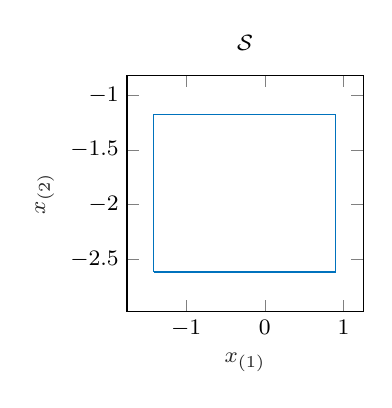
\begin{tikzpicture}
\footnotesize

\begin{axis}[%
width=3cm,
height=3cm,
at={(0in,0in)},
scale only axis,
xmin=-1.75,
xmax=1.25,
xlabel style={font=\color{white!15!black}},
xlabel={$x_{(1)}$},
ymin=-2.98,
ymax=-0.82,
ylabel style={font=\color{white!15!black}},
ylabel={$x_{(2)}$},
axis background/.style={fill=white},
title style={font=\bfseries},
title={$\mathcal{S}$}
]
\addplot [color=mycolor1, forget plot]
  table[row sep=crcr]{%
-1.4113	-2.6153\\
0.8993	-2.6153\\
0.8993	-1.1773\\
-1.4113	-1.1773\\
-1.4113	-2.6153\\
};
\end{axis}
\end{tikzpicture}%
\end{minipage}
\begin{minipage}[t]{0.25\textwidth}
	\vspace{10pt}

	\begin{verbatim}
	Command Window:
		
	S = 
  [-1.4113, 0.8993]
  [-2.6153, -1.1773]
	\end{verbatim}
\end{minipage}
\begin{minipage}[t]{0.3\textwidth}
	\vspace{0pt}
	\centering
	\includetikz{./figures/tikz/set-operations-aux/example_generateRandom}
\end{minipage}
\end{center}

\vspace{1cm}

\subsubsubsection{linComb}
\label{sec:linComb}

The method \operator{linComb} implements the linear combination of two sets. Given two sets $\mathcal{S}_1,\mathcal{S}_2 \subset \Rn$, their linear combination is defined as 
\begin{equation*}
	\operator{linComb}(\mathcal{S}_1,\mathcal{S}_2) = \left \{ \lambda s_1 + (1-\lambda) s_2 ~|~ s_1 \in \mathcal{S}_1,~s_2 \in \mathcal{S}_2,~\lambda \in [0,1] \right\}.
\end{equation*}
Note that for convex sets the linear combination is identical to the convex hull (see \cref{sec:convHull}). For non-convex sets, however, the two operations differ.
Let us demonstrate the method $\operator{linComb}$ by an example:

\begin{center}
\begin{minipage}[t]{0.38\textwidth}
	\vspace{10pt}
	\footnotesize
	\input{./MATLABcode/example_linComb}
\end{minipage}
\begin{minipage}[t]{0.6\textwidth}
	\vspace{0pt}
	\centering
	\includetikz{./figures/tikz/set-operations-aux/example_linComb}
\end{minipage}
\end{center}

\subsubsubsection{randPoint}

The method \operator{randPoint} returns random points located inside a set. Given a set $\mathcal{S} \subset \Rn$, the method \operator{randPoint} generates random points $p = [p_1,\dots,p_N] \in \R^{n \times N}$ with $p_1,\dots, p_N \in \mathcal{S}$:
\begin{equation*}
	\begin{split}
		& p = \operator{randPoint}(\mathcal{S}), \\
		& p = \operator{randPoint}(\mathcal{S},N), \\
		& p = \operator{randPoint}(\mathcal{S},N,\texttt{type}),
   \end{split}
\end{equation*}
where $N \in \mathbb{N}_{> 0}$ is the desired number of points, and \texttt{type} specifies the desired type random points. The setting \texttt{type = 'extreme'} aims to generate points close to or on the boundary of the set, while \texttt{type = 'standard'} generates arbitrary points within the set. In contrast, the setting \texttt{type = 'uniform'} generates uniformly distributed points within the set, potentially at the cost of a longer runtime. The default values are $N = 1$ and \texttt{type = 'standard'}. Let us demonstrate the method \operator{randPoint} by an example:

\begin{center}
\begin{minipage}[t]{0.40\textwidth}
	\vspace{10pt}
	\footnotesize
	% This file was created by matlab2tikz.
%
\definecolor{mycolor1}{rgb}{0.00000,0.44700,0.74100}%
%
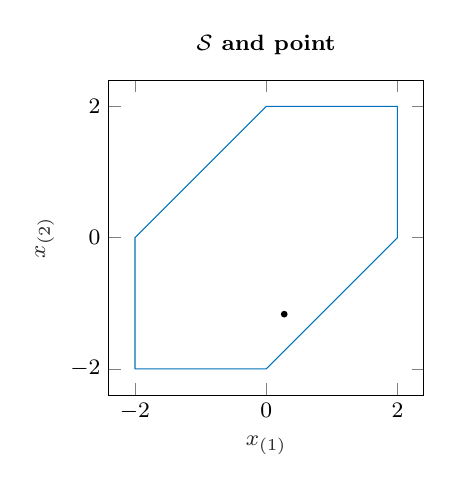
\begin{tikzpicture}
\footnotesize

\begin{axis}[%
width=4cm,
height=4cm,
at={(0in,0in)},
scale only axis,
xmin=-2.4,
xmax=2.4,
xlabel style={font=\color{white!15!black}},
xlabel={$x_{(1)}$},
ymin=-2.4,
ymax=2.4,
ylabel style={font=\color{white!15!black}},
ylabel={$x_{(2)}$},
axis background/.style={fill=white},
title style={font=\bfseries},
title={$\mathcal{S}$ and point}
]
\addplot [color=mycolor1, forget plot]
  table[row sep=crcr]{%
-2	-2\\
0	-2\\
2	0\\
2	2\\
0	2\\
-2	0\\
-2	-2\\
};
\addplot[only marks, mark=*, mark options={}, mark size=1.0000pt, draw=black, forget plot] table[row sep=crcr]{%
x	y\\
0.2747	-1.1657\\
};
\end{axis}
\end{tikzpicture}%
\end{minipage}
\begin{minipage}[t]{0.2\textwidth}
	\vspace{10pt}

	\begin{verbatim}
	Command Window:
		
	p =

    0.2747
   -1.1657
	\end{verbatim}
\end{minipage}
\begin{minipage}[t]{0.3\textwidth}
	\vspace{0pt}
	\centering
	\includetikz{./figures/tikz/set-operations-aux/example_randPoint}
\end{minipage}
\end{center}

\vspace{1cm}

\subsubsubsection{reduce}

The method \operator{reduce} encloses a set by another set with a smaller representation size. Given a set $\mathcal{S} \subset \Rn$, the method \operator{reduce} computes
\begin{equation}
	\operator{reduce}(\mathcal{S},\texttt{method},\texttt{order}) = \overline{\mathcal{S}}, ~~~ \mathcal{S} \subseteq \overline{\mathcal{S}},
	\label{eq:reduce}
\end{equation}
where the representation size of $\overline{\mathcal{S}}$ is smaller than the one of $\mathcal{S}$. The parameter \texttt{method} in \eqref{eq:reduce} is a string that specifies the algorithm to be applied, see \cref{tab:zono_reduction}. The parameter \texttt{order} in \eqref{eq:reduce} is a measure for the desired representation size of the resulting set $\overline{\mathcal{S}}$. Currently, the method \operator{reduce} is implemented for the zonotopic set representations \texttt{zonotope} (see \cref{sec:zonotope}), \texttt{conZonotope} (see \cref{sec:conZonotope}), \texttt{polyZonotope} (see \cref{sec:polynomialZonotopes}), and \texttt{probZonotope} (see \cref{sec:probabilisticZonotopes}), where $\texttt{order} = \frac{p}{n}$ is defined as the division of the number of generator vectors $p$ by the system dimension $n$. Let us demonstrate the method \operator{reduce} by an example:

\begin{center}
\begin{minipage}[t]{0.35\textwidth}
	\vspace{10pt}
	\footnotesize
	\input{./MATLABcode/example_reduce}
\end{minipage}
\begin{minipage}[t]{0.6\textwidth}
	\vspace{0pt}
	\centering
	\includetikz{./figures/tikz/set-operations-aux/example_reduce}
\end{minipage}
\end{center}


\begin{table}[h]
	\caption{Reduction techniques for zonotopic set representations.}
	\centering
	\label{tab:zono_reduction}
	\begin{tabular}{lll}
		\toprule
		\textbf{Technique} & \textbf{Primary use} & \textbf{Reference} \\
		\midrule
		\texttt{cluster} & Reduction to low order by clustering generators & \cite[Sec.~III.B]{Kopetzki2017} \\
		\texttt{combastel} & Reduction of high to medium order & \cite[Sec.~3.2]{Combastel2003} \\
		\texttt{constOpt} & Reduction to low order by optimization & \cite[Sec.~III.D]{Kopetzki2017} \\
		\texttt{girard} & Reduction of high to medium order & \cite[Sec. ~.4]{Girard2005} \\
		\texttt{methA} & Reduction to low order by volume minimization (A) & Meth. A, \cite[Sec.~2.5.5]{Althoff2010a} \\
		\texttt{methB} & Reduction to low order by volume minimization (B) & Meth. B, \cite[Sec.~2.5.5]{Althoff2010a} \\
		\texttt{methC} & Reduction to low order by volume minimization (C) & Meth. C, \cite[Sec.~2.5.5]{Althoff2010a} \\
		\texttt{scott} & Reduction to low order  & \cite[Appendix]{Scott2016} \\
		\texttt{pca} & Reduction of high to medium order using PCA & \cite[Sec.~III.A]{Kopetzki2017} \\
		\bottomrule
	\end{tabular}
\end{table}


\subsubsubsection{supportFunc}

The method \operator{supportFunc} computes the support function for a specific direction. Given a set $\mathcal{S} \in \Rn$ and a vector $l \in \Rn$, the support function is defined as
\begin{equation*}
	\operator{supportFunc}(\mathcal{S},l) = \max_{x \in \mathcal{S}} ~l^T~x.
\end{equation*}
The function also supports the computation of the lower bound, which can be calculated using the flag \texttt{'lower'}:
\begin{equation*}
	\operator{supportFunc}(\mathcal{S},l,\texttt{'lower'}) = \min_{x \in \mathcal{S}} ~l^T~x.
\end{equation*}
Additionally, one can return both the lower and upper bounds by using the flag \texttt{'range'}.
Let us demonstrate the method \operator{supportFunc} by an example:

\begin{center}
\begin{minipage}[t]{0.40\textwidth}
	\vspace{10pt}
	\footnotesize
	% This file was created by matlab2tikz.
%
\definecolor{mycolor1}{rgb}{0.00000,0.44700,0.74100}%
\definecolor{mycolor2}{rgb}{0.85000,0.32500,0.09800}%
%
\begin{tikzpicture}
\footnotesize

\begin{axis}[%
width=4cm,
height=4cm,
at={(0in,0in)},
scale only axis,
xmin=-2.5,
xmax=2.5,
xlabel style={font=\color{white!15!black}},
xlabel={$x_{(1)}$},
ymin=-2.5,
ymax=2.5,
ylabel style={font=\color{white!15!black}},
ylabel={$x_{(2)}$},
axis background/.style={fill=white},
title style={font=\bfseries},
title={$\mathcal{S}$ and \texttt{supportFunc}}
]
\addplot [color=mycolor1, forget plot]
  table[row sep=crcr]{%
-2	-2\\
0	-2\\
2	0\\
2	2\\
0	2\\
-2	0\\
-2	-2\\
};
\addplot [color=mycolor2, forget plot]
  table[row sep=crcr]{%
2.5	1.75\\
1	2.5\\
};
\end{axis}
\end{tikzpicture}%
\end{minipage}
\begin{minipage}[t]{0.2\textwidth}
	\vspace{10pt}

	\begin{verbatim}
	Command Window:
		
	res = 6
	\end{verbatim}
\end{minipage}
\begin{minipage}[t]{0.3\textwidth}
	\vspace{0pt}
	\centering
	\includetikz{./figures/tikz/set-operations-aux/example_supportFunc}
\end{minipage}
\end{center}


\subsubsubsection{plot}

The method \operator{plot} visualizes a 2-dimensional projection of the boundary of a set. Given a set $\mathcal{S} \subset \Rn$, the method \operator{plot} supports the following syntax:
\begin{equation*}
	\begin{split}
		&\texttt{han} = \operator{plot}(\mathcal{S}), \\
		&\texttt{han} = \operator{plot}(\mathcal{S},\texttt{dims}), \\
		&\texttt{han} = \operator{plot}(\mathcal{S},\texttt{dims},\texttt{linespec}), \\
		&\texttt{han} = \operator{plot}(\mathcal{S},\texttt{dims},\texttt{namevaluepairs}), \\
	\end{split}
\end{equation*}
where \texttt{han} is a handle to the plotted MATLAB graphics object and the additional input arguments are defined as

\begin{itemize}
	\item \texttt{dims}: Integer vector $\texttt{dims} \in \mathbb{N}_{\leq n}^2$ specifying the dimensions for which the projection is visualized (default value: \texttt{dim = [1 2]}).
	\item \texttt{linespec}: (optional) line specifications, e.g., \texttt{'--*r'}, as supported by MATLAB\footnote{\url{https://de.mathworks.com/help/matlab/ref/linespec.html}}.
	\item \texttt{namevaluepairs}: (optional) further specifications as name-value pairs, e.g.,
	\texttt{'LineWidth',2} and \texttt{'FaceColor',[.5 .5 .5]}, as supported by MATLAB.
	If the plot is not filled, these are the built-in
	Line Properties\footnote{\url{https://de.mathworks.com/help/matlab/ref/matlab.graphics.chart.primitive.line-properties.html}},
	if the plot is filled, they correspond to the Patch Properties\footnote{\url{https://de.mathworks.com/help/matlab/ref/matlab.graphics.primitive.patch-properties.html}}.
\end{itemize}

Let us demonstrate the method  \operator{plot} by an example:

\begin{center}
\begin{minipage}[t]{0.40\textwidth}
	\vspace{10pt}
	\footnotesize
	\input{./MATLABcode/example_plot}
\end{minipage}
\begin{minipage}[t]{0.3\textwidth}
	\vspace{0pt}
	\centering
	\includetikz{./figures/tikz/set-operations-aux/example_plot}
\end{minipage}
\end{center}


\vspace{1cm}

\subsubsubsection{project}

The method \operator{project} projects a set to a lower-dimensional, axis-aligned subspace. Given a set $\mathcal{S} \subset \Rn$ and a vector of subspace indices $\texttt{dims} \in \mathbb{N}_{\leq n}^m$, the method \operator{project} returns
\begin{equation*}
	\operator{project}(\mathcal{S},\texttt{dims}) = \Big \{ [s_{(\texttt{dims}_{(1)})},\dots,s_{(\texttt{dims}_{(m)})}]^T ~\Big |~ s \in \mathcal{S} \Big \} \subset \R^m,
\end{equation*}
where $s_{(i)}$ denotes the i-th entry of vector $s$. Let us demonstrate the method  \operator{project} by an example:

\begin{center}
\begin{minipage}[t]{0.40\textwidth}
	\vspace{10pt}
	\footnotesize
	\input{./MATLABcode/example_project}
\end{minipage}
\begin{minipage}[t]{0.25\textwidth}
	\vspace{10pt}

	\begin{verbatim}	
	Command Window:
	
	res = 
 [1.00000,3.00000]
 [5.00000,7.00000]
 [0.00000,2.00000]
	\end{verbatim}
\end{minipage}
\end{center}

A set can be projected into a higher-dimensional space using the function \operator{projectHighDim},
where the new dimensions are bounded at 0.
On the other hand, the function \operator{lift} lifts the set into a higher-dimensional space with unbounded new dimensions.

